\documentclass[presentation]{beamer}
\usetheme{CambridgeUS}
\usecolortheme{orchid}

\definecolor{themeColor}{HTML}{4e6eff}

\setbeamercolor*{structure}{bg=black,fg=themeColor}

\setbeamercolor*{palette primary}{use=structure,fg=white,bg=structure.fg}
\setbeamercolor*{palette secondary}{use=structure,fg=white,bg=structure.fg!75}
\setbeamercolor*{palette tertiary}{use=structure,fg=white,bg=structure.fg!50!black}
\setbeamercolor*{palette quaternary}{fg=white,bg=black}

\setbeamercolor{section in toc}{fg=black,bg=white}
\setbeamercolor{alerted text}{use=structure,fg=structure.fg!50!black!80!black}

\setbeamercolor{titlelike}{parent=palette primary,fg=structure.fg!50!black}
\setbeamercolor{frametitle}{bg=structure.fg!10!white,fg=structure.fg!50!black!80!black}

\setbeamercolor*{titlelike}{parent=palette primary}


\usepackage[T1]{fontenc}
\usepackage[utf8]{inputenc}
\usepackage{amssymb}
\usepackage{graphicx}
\usepackage{subfigure}
\usepackage{multirow}
\usepackage{hhline}
\usepackage{amsfonts,amstext,amssymb,wasysym}
\usepackage{fancyvrb}
\usepackage{alltt}
\usepackage{textcomp}
\usepackage{url}
\usepackage{multimedia,pgf}
\usepackage{geometry}
\usepackage{minted}
\usepackage{bibentry}
\usepackage{framed}
\usepackage{pmboxdraw}
\usepackage{newunicodechar}
\newunicodechar{└}{\textSFii}
\newunicodechar{├}{\textSFviii}
\newunicodechar{─}{\textSFx}
\usepackage{cleveref}
\nobibliography*

\title[03 - Dependency Management]{\small{\input{../coursetitle}} \\
\normalsize{Enforce reproducibility: dependency management and build automation}}

% ! TeX root = 01-Introduction/01-Introduction.tex
\author[D. Pianini]{
Danilo Pianini\\
\texttt{{\footnotesize danilo.pianini@unibo.it}}}

\institute[UniBo]
{\textsc{Alma Mater Studiorum}---Universit\`a di Bologna}

\date[\today{}]{\input{../context} \\
\scriptsize \input{../date} - \input{../place} 
}

\pgfdeclareimage[height=0.625cm]{university-logo}{../images/logo}
\logo{\pgfuseimage{university-logo}}


\newcommand{\codefile}[4]{
	\begin{block}{\texttt{#2}}
		\inputminted[fontsize=#3,linenos=true,breaklines=true]{#4}{"workspace/#1/#2"}
	\end{block}
}
\newcommand{\java}[3]{\codefile{#1}{#2}{#3}{java}}
\newcommand{\ccode}[3]{\codefile{#1}{#2}{#3}{c}}
\newcommand{\cpp}[3]{\codefile{#1}{#2}{#3}{cpp}}
\newcommand{\groovy}[3]{\codefile{#1}{#2}{#3}{groovy}}
\newcommand{\kotlin}[3]{\codefile{#1}{#2}{#3}{kotlin}}
\newcommand{\scala}[3]{\codefile{#1}{#2}{#3}{scala}}
\newcommand{\python}[3]{\codefile{#1}{#2}{#3}{python}}
\newcommand{\markdown}[3]{\codefile{#1}{#2}{#3}{markdown}}
\newcommand{\terminal}[3]{\codefile{#1}{#2}{#3}{text}}

\newcommand{\tinier}{\fontsize{4pt}{5pt}\selectfont}
\newcommand{\fnurl}[1]{\footnote{\url{#1}}}

\begin{document}

% ! TeX root = 01-Introduction/01-Introduction.tex
\AtBeginSubsection[]{%
  \begin{frame}<beamer>
    \frametitle{Outline}
    \tableofcontents[currentsection,currentsubsection]
  \end{frame}
  \addtocounter{framenumber}{-1}% If you don't want them to affect the slide number
}


%===============================================================================
\frame[label=coverpage]{\titlepage}
%===============================================================================

%===============================================================================
%===============================================================================
\section*{Outline}
%===============================================================================
%===============================================================================

\frame{\tableofcontents}

%===============================================================================
%===============================================================================

\section{Dependency Management}

\subsection{Concept}
\begin{frame}[fragile]{The concept of dependency}
  \begin{itemize}
    \item Any software \textbf{depends} on other software
    \begin{itemize}
      \item All the runtime base libraries (think of \texttt{java.lang.* and System.*})
      \item All the other core libraries
      \item Possibly, external resources (e.g., images, sounds, translation files...)
    \end{itemize}
   \item Normally, this software depends on other software
    \begin{itemize}
      \item That depend on other software
		\begin{itemize}
			\item That depend on other software, and so on...
		\end{itemize}
    \end{itemize}
   \item A normal applications has a \textbf{tree} of dependencies
  \end{itemize}
\end{frame}

\subsection{Example}
\begin{frame}[fragile]{Example: print titles}
	\begin{block}{Requirements}
		Write a program that:
		\begin{itemize}
			\item Visits TheTVDB.org (public TV Series database)
			\item Searches for a series
			\item Download the titles of all the episodes
			\item Prints them on screen
		\end{itemize}
	\end{block}
	\begin{block}{Questions}
		\begin{itemize}
			\item Estimate how much code you'd need to write
			\item How much code can be just inherited from existing, public libraries?
		\end{itemize}
	\end{block}
\end{frame}

\begin{frame}[fragile]{Maybe less code than you may expect}
	\kotlin{01-dependencies}{src/main/kotlin/it/unibo/ci/PrintSeries.kt}{\tiny}
\end{frame}

\begin{frame}[fragile]{Trick revealed}
  I used a few existing libraries!
  \begin{itemize}
    \item Kotlin standard library
    \begin{itemize}
      \item Easy manipulation of resources
    \end{itemize}
    \item Omertron's thetvdbapi
    \begin{itemize}
      \item Queries TheTVDB given a valid API key, hiding all the HTTP communication and XML parsing
    \end{itemize}
  \end{itemize}
  \begin{block}{But wait, there is more!}
    I only needed three libraries to get the job done. But are those libraries using other libraries?
  \end{block}
\end{frame}

\subsection{Dependency trees}
\begin{frame}[fragile]{The actual dependency tree (for compiling)}
  \begin{block}{}
    \begin{minted}[fontsize=\scriptsize]{bash}
+--- org.jetbrains.kotlin:kotlin-stdlib:1.3.50
|    +--- org.jetbrains.kotlin:kotlin-stdlib-common:1.3.50
|    \--- org.jetbrains:annotations:13.0
\--- com.omertron:thetvdbapi:[1.6, 1.7] -> 1.7
     +--- org.slf4j:slf4j-api:1.7.9
     \--- org.yamj:api-common:1.2
          +--- org.apache.commons:commons-lang3:3.3.2
          +--- commons-dbcp:commons-dbcp:1.4
          |    \--- commons-pool:commons-pool:1.5.4 -> 1.6
          +--- commons-pool:commons-pool:1.6
          +--- commons-codec:commons-codec:1.10
          +--- org.apache.httpcomponents:httpclient:4.3.6
          |    +--- org.apache.httpcomponents:httpcore:4.3.3
          |    +--- commons-logging:commons-logging:1.1.3
          |    \--- commons-codec:commons-codec:1.6 -> 1.10
          \--- org.slf4j:slf4j-api:1.7.9
    \end{minted}
  \end{block}
  \begin{itemize}
   \item Libraries depend on other libraries
   \item All the libraries must be in the classpath!
   \item Runtime libraries may differ from compile libraries!
  \end{itemize}
\end{frame}

\begin{frame}[fragile]{The actual dependency tree (for runtime)}
  \begin{block}{}
    \begin{minted}[fontsize=\scriptsize]{bash}
+--- org.jetbrains.kotlin:kotlin-stdlib:1.3.50
|    +--- org.jetbrains.kotlin:kotlin-stdlib-common:1.3.50
|    \--- org.jetbrains:annotations:13.0
+--- com.omertron:thetvdbapi:[1.6, 1.7] -> 1.7
|    +--- org.slf4j:slf4j-api:1.7.9
|    \--- org.yamj:api-common:1.2
|         +--- org.apache.commons:commons-lang3:3.3.2
|         +--- commons-dbcp:commons-dbcp:1.4
|         |    \--- commons-pool:commons-pool:1.5.4 -> 1.6
|         +--- commons-pool:commons-pool:1.6
|         +--- commons-codec:commons-codec:1.10
|         +--- org.apache.httpcomponents:httpclient:4.3.6
|         |    +--- org.apache.httpcomponents:httpcore:4.3.3
|         |    +--- commons-logging:commons-logging:1.1.3
|         |    \--- commons-codec:commons-codec:1.6 -> 1.10
|         \--- org.slf4j:slf4j-api:1.7.9
\--- javax.xml.ws:jaxws-api:+ -> 2.3.1
     +--- javax.xml.bind:jaxb-api:2.3.1
     |    \--- javax.activation:javax.activation-api:1.2.0
     +--- javax.xml.soap:javax.xml.soap-api:1.4.0
     \--- javax.annotation:javax.annotation-api:1.3.2
    \end{minted}
  \end{block}
\end{frame}

\subsection{Preventing dependency hells}
\begin{frame}[fragile, allowframebreaks]{Towards a dependency hell}
	This was a toy program, consisting of a single source file of few lines of code.

	Regardless, it requires \textbf{20} external libraries in order to run.
	
	\begin{block}{Libraries explosion}
		\begin{itemize}
			\item It is very common for a non-toy project to get past 100 dependencies
			\begin{itemize}
				\item Alchemist, big but not huge, counts more than 330 dependencies
				\item (and that's runtime \textbf{alone})
			\end{itemize}
			\item Hard to search, download and verify compatibilities by hand 
			\item Version conflicts soon arise
			\begin{itemize}
				\item one of your direct dependencies uses library \texttt{A} at version 1
				\item another uses library \texttt{A} at version 2
				\item you have a so-called transitive dependency conflict on \texttt{A}
			\end{itemize}
			\item Upgrading by hand requires, time, effort and tons of testing
		\end{itemize}
	\end{block}
	\begin{block}{Source import}
		\begin{itemize}
			\item Duplication
			\item More library code than product code
			\item Extremely difficult to update
			\item Style inconsistencies
			\item Different quality metrics
			\item Duplication
			\item Unmaintainable
		\end{itemize}
	\end{block}
	\begin{block}{Binary import (copy of so/dll/jar in the repo)}
		\begin{itemize}
			\item At every update, a new jar must be included, along with all its dependencies
			\item Being a compressed binary file, its hard to write diffs
			\item Git must store a copy of the file for each version (even if very little changed actually)
			\item The repository size explodes
			\begin{itemize}
				\item Take a look at \cite{explodedrepository} for an anti-pattern
			\end{itemize}
		\end{itemize}
	\end{block}
	\begin{block}{}
		Trust me, you want an automated tool to get you out of this hell.
	\end{block}
\end{frame}

\begin{frame}[fragile]{Desiderata}
	\begin{itemize}
		\item Declarative dependency specification
		\item Automatic fetch and retrieve of the required dependencies
		\item Automatic and configurable version conflict resolution
		\item Multiple dependency scopes:
		\begin{itemize}
			\item We need JUnit for our tests, but we don't want any of our production sources to use its APIs (test scope differs from compile scope)
			\item also, we don't want to embed JUnit in our production dependency set (test scope differs from runtime scope)
			\item We need Logback \cite{logback} for our runtime, but we want our code to depend only on the SLF4J APIs for reusability (runtime scope larger than compile scope)
			\item We want ANTLR4 \cite{antlr4} for generating some source code, but we only want its runtime once this phase is concluded (custom scope)
		\end{itemize}
		\item Configurable software sources
	\end{itemize}
\end{frame}

\begin{frame}[fragile]{Possible desired code}
  \begin{block}{}
    \begin{minted}[fontsize=\scriptsize]{kotlin}
// Where to find software packets
repositories {
    mavenCentral()
    jCenter()
}
// Which software packets we need in each lifecycle phase
dependencies {
    // Generating sources
    sourceGeneration("org.antlr:antlr4:4.7")
    // Packets of which we inherit the API
    api("org.slf4j:slf4j-api:1.7.25")
    // Stuff we use for implementing our own stuff
    implementation("org.antlr:antlr-runtime:3.5.2")
    testImplementation("junit:junit:4.12") // Implementing tests
    // Stuff we use at runtime, but with no compile dependency towards
    runtimeOnly("ch.qos.logback:logback-classic:1.2.2")
    // Stuff we use only when running tests
    testRuntimeOnly("ch.qos.logback:logback-classic:1.2.2")
}
    \end{minted}
  \end{block}
\end{frame}

\section{Build automation}

\begin{frame}[fragile]{Moar automation}
	Dependency management is just the \textit{first} need that arises.
	
	\begin{block}{What you really want to automatize}
		\begin{itemize}
			\item Dependency management
			\item Software compilation
			\item Testing
			\item Documentation generation
			\item Reports generation
			\item Artefacts assemblage
			\item Artefacts signing
		\end{itemize}
	\end{block}
	\begin{itemize}
		\item Everything that goes from declaring what your software needs to having it ready for deployment
		\item Except actually \textit{developing} the project
	\end{itemize}
\end{frame}

\begin{frame}{Imperative style}
    \begin{block}{Instructions on \textit{what to do}}
        \begin{itemize}
            \item No explicit convention
            \item Very high flexibility
            \item Easy to customize in depth
            \item High duplication among projects with similar conventions
            \item Hard to get started with a ``standard'' project
            \item Often does not deal with dependencies (they are typically declarative)
        \end{itemize}
    \end{block}
    \begin{block}{Examples}
        \begin{itemize}
            \item Custom scripts (in bash or similar languages)
            \item CMake
            \item Apache Ant
        \end{itemize}
    \end{block}
\end{frame}
\begin{frame}{Declarative style}
    \begin{block}{A configuration with a the \textit{settings} of the project}
        \begin{itemize}
            \item Default configuration based on a convention
            \item Low flexibility
            \item Hard to customize in depth
            \begin{itemize}
                \item Custom behaviour must be implemented separately, e.g. as plugin
            \end{itemize}
            \item Low duplication among projects following the convention
            \item Very easy to get started with a conventional project
        \end{itemize}
    \end{block}
    \begin{block}{Examples}
        \begin{itemize}
            \item Apache Ivy (dependencies only)
            \item Apache Maven
            \item Python pip
        \end{itemize}
    \end{block}
\end{frame}

\subsection{Introduction to Gradle}

\begin{frame}[fragile, allowframebreaks]{Gradle}
	\begin{block}{Idea}
		Pick the best of ``declarative'' build systems, such as Apache Maven
		\begin{itemize}
			\item Dependency resolution
			\item Conventions for easily building ``standard'' projects
			\item Extensibility by plugin
		\end{itemize}
		Pick the best from ``imperative'' build systems, such as Apache Ant.
		\begin{itemize}
			\item Extreme flexibility
			\item Customization by scripting
		\end{itemize}
	\end{block}
	\begin{block}{Features in a box}
		\begin{itemize}
			\item The build is written in Domain Specific Language
			\begin{itemize}
			    \item Groovy is the historical hosting language
			    \item Kotlin is the modern alternative (we are going to use this one)
			\end{itemize}
			\item Inherits from Ant the concept of ``target'' (renamed as ``task'')
			\item Automagic resolution of the order in which tasks should be executed
			\item Built-in dependency resolution as Maven (SBT and Ant rely on Apache Ivy)
			\item Incremental builds and parallel task execution
			\item Supports many languages
			\begin{itemize}
                \item Java, Scala, Groovy, Kotlin, and C/C++ are first class citizens
                \item Others supported via plugin
			\end{itemize}
			\item Maven-style extensibility via plugins
		\end{itemize}
	\end{block}
	\begin{block}{Diffusion}
		\begin{itemize}
			\item Replacing Ant+Ivy and Maven as reference build system for Java and other JVM based languages
			\item Gaining momentum also in the C/C++ community (assembler, c, cpp, objective-c, and objective-cpp are set to be included in the base distribution)
			\item Selected by Google as preferred build system for Android
			\begin{itemize}
				\item Android Studio by default configures a Gradle build under the hood
			\end{itemize}
			\item Well integrated in several IDEs (Eclipse, IntelliJ, Visual Studio, XCode)
		\end{itemize}
	\end{block}
	\begin{block}{Details}
		\begin{itemize}
			\item Created in 2008 by Gradleware
			\item Mostly implemented in Java 5, with an outer layer in Groovy
			\item Free - both as in freedom (Apache License 2.0) and as in beer (no fees required)
			\item Source code available on GitHub
			\item Thorough documentation - though some advanced use requires some good personal initiative...
		\end{itemize}
	\end{block}
\end{frame}

\begin{frame}[fragile]{Under the hood}
	\begin{itemize}
		\item The Gradle build script is a valid Kotlin script (if you consider the Gradle API)
		\item Anything with invalid Kotlin syntax is not a valid Gradle build script
		\item Kotlin syntax allows for ``internal'' DSLs, Gradle leverages this feature
		\item Everything you write is actually proper Kotlin code (method calls, closures, and so on), and you can leverage the language features to customize your build as well
		\item At the high level, the feeling is to just have to configure an existing plugin, much like Maven, for most of the things you normally do
		\item When needed, it is easy to configure custom behavior, or fiddle with the internals, in a functional or imperative fashion
	\end{itemize}
\end{frame}

\subsection{Gradle basics}

\begin{frame}[fragile]{Gradle concepts}
	\begin{block}{Project - from the Gradle documentation}
			What a project represents depends on what it is that you are doing with Gradle. For example, a project might represent a library JAR or a web application. It might represent a distribution ZIP assembled from the JARs produced by other projects. \\
			A project does not necessarily represent a thing to be built.
			It might represent a thing to be done, such as deploying your application to staging or production environments.
	\end{block}
	\begin{block}{Task - from the Gradle documentation}
			Each project is made up of one or more tasks. \\
			A task represents some atomic piece of work which a build performs.\\
			This might be compiling some classes, creating a JAR, generating Javadoc, or publishing some archives to a repository.
	\end{block}
\end{frame}

\begin{frame}[fragile,allowframebreaks]{My first Gradle build}
    \begin{block}{Takeaways}
        A Gradle build is configured in:
        \begin{itemize}
            \item the \texttt{build.gradle.kts} file for Kotlin-based build scripts.
            \item the \texttt{build.gradle} file for Groovy-based build scripts.
        \end{itemize}
    \end{block}
    \kotlin{02-SimpleTask}{build.gradle.kts}{\normalsize}
    \terminal{02-SimpleTask}{gradle tasks --all}{\tinier} 
    \terminal{02-SimpleTask}{gradle hello}{\normalsize}
\end{frame}

\begin{frame}[fragile,allowframebreaks]{Build scripts are code}
    \begin{block}{Takeaways}
        \begin{itemize}
            \item Kotlin can be fully exploited to write programs inside your build script
            \item Existing tasks can be modified
            \item Arbitrary operations can be (pre-/ap-)pended to existing tasks
        \end{itemize}
    \end{block}
    \kotlin{03-BuildAsCode}{build.gradle.kts}{\normalsize}
    \terminal{03-BuildAsCode}{gradle hello}{\normalsize}
\end{frame}

\begin{frame}[fragile,allowframebreaks]{Task dependencies}
    \begin{block}{Takeaways}
        \begin{itemize}
            \item Tasks depends on other tasks
            \item Dependencies can be defined manually
            \item Dependencies can be defined lazily (for tasks that do not yet exist)
            \item Dependencies can be defined at task definition or later
            \item Gradle resolves dependencies automatically
        \end{itemize}
    \end{block}
    \kotlin{04-TaskDependencies}{build.gradle.kts}{\scriptsize}
    \terminal{04-TaskDependencies}{gradle tasks --all}{\tinier}
    \terminal{04-TaskDependencies}{gradle complete}{\normalsize}
\end{frame}

\begin{frame}[fragile,allowframebreaks]{Dynamic tasks}
    \begin{block}{Takeaways}
        \begin{itemize}
            \item Tasks can be created programmatically
            \item The \texttt{-q} flag quietens the output
        \end{itemize}
    \end{block}
    \kotlin{05-DynamicTasks}{build.gradle.kts}{\scriptsize}
    \terminal{05-DynamicTasks}{gradle -q task42}{\normalsize}
\end{frame}

\begin{frame}[fragile,allowframebreaks]{Using plugins}
    \begin{block}{Takeaways}
        \begin{itemize}
            \item A plugin extends the functionality of Gradle
            \item A huge number of plugins exist
            \begin{itemize}
                \item see: \url{https://plugins.gradle.org/}
            \end{itemize}
            \item Once applied, tasks and configurations introduced by the plugin are available for the buildscript
            \item Plugins can be written quite easily
            \begin{itemize}
                \item Documentation is good
                \item If you have many similar projects, it may be way better to write your own plugin rather than copypasting the build script
                \item I wrote \href{several plugins myself}{https://plugins.gradle.org/search?term=org.danilopianini}...
            \end{itemize}
        \end{itemize}
    \end{block}
    \kotlin{08-Plugin}{build.gradle.kts}{\scriptsize}
    \terminal{08-Plugin}{gradle tasks --all}{\tiny}
    \terminal{08-Plugin}{gradle hello}{\tinier}
\end{frame}

\begin{frame}[fragile,allowframebreaks]{Properties}
    \begin{block}{Takeaways}
        \begin{itemize}
            \item Tasks don't accept parameters
            \item Tasks can access project variables
            \item Variables can be passed through the command line with the \texttt{-P} option
            \item Variables can be set in an ancillary \texttt{gradle.properties} file
        \end{itemize}
    \end{block}
    \groovy{09-Properties}{build.gradle}{\scriptsize}
    \terminal{09-Properties}{gradle.properties}{\scriptsize}
    \terminal{09-Properties}{gradle printProperties -PpropertyFromCLI='defined in the CLI'}{\normalsize}
\end{frame}

\begin{frame}[fragile,allowframebreaks]{Setting a project name}
    \begin{block}{Takeaways}
        \begin{itemize}
            \item If no project name is set, the project will be named after the enclosing folder            \item The project name (and other settings) can be controlled by changing \texttt{settings.gradle}
            \item \texttt{settings.gradle} can refer to variables defined in \texttt{gradle.properties}
        \end{itemize}
    \end{block}
    \groovy{10-ProjectName}{build.gradle}{\scriptsize}
    \terminal{10-ProjectName}{gradle.properties}{\scriptsize}
    \terminal{10-ProjectName}{settings.gradle}{\scriptsize}
    \terminal{10-ProjectName}{gradle projectName}{\scriptsize}
\end{frame}

\begin{frame}[fragile,allowframebreaks]{Organising tasks}
    \begin{block}{Takeaways}
        \begin{itemize}
            \item Tasks can be set a group and a description
        \end{itemize}
    \end{block}
    \terminal{11-TaskDescription}{settings.gradle}{\scriptsize}
    \terminal{11-TaskDescription}{gradle.properties}{\scriptsize}
    \groovy{11-TaskDescription}{build.gradle}{\scriptsize}
    \terminal{11-TaskDescription}{gradle tasks}{\tinier}
\end{frame}

\begin{frame}[fragile,allowframebreaks]{The build system as dependency}
    \begin{block}{The build system \textit{is a dependency}}
        \begin{itemize}
            \item We said that a dependency is any software that we need to make our own work
            \item Making it work includes compiling and packaging it
            \item A change in the build system would impact our product!
            \item \textbf{The build system and its configuration are dependencies of our projects!}
        \end{itemize}
    \end{block}
    \begin{block}{A circular problem}
        \begin{itemize}
            \item We cannot build until all the dependencies are satisfied
            \item We want to use the build system to specify dependencies
            \item But the build system is a ultimately a dependency...
        \end{itemize}
    \end{block}
    \begin{block}{Possible solution: the Gradle wrapper}
        \begin{itemize}
            \item Provide a minimal script that:
            \begin{itemize}
                \item Downloads the \textit{exact version} of Gradle for which the build was written
                \item Installs it
                \item Executes the build using such build tool
            \end{itemize}
            \item Gradle has the capability of generating its own wrapper
            \begin{itemize}
                \item \texttt{gradle wrapper --gradle-version 4.7}
                \item Generates all the base files required for wrapping Gradle 4.7
                \item In case the version is unspecified, the currently installed Gradle version is used
            \end{itemize}
            \item The wrapper generates:
            \begin{itemize}
                \item A \texttt{gradlew} bash script for Unix systems
                \item A \texttt{gradlew.bat} batch file for Windows systems
                \item A \texttt{gradle} folder containing a core jar and metadata
            \end{itemize}
        \end{itemize}
    \end{block}
    \begin{block}{The Gradle wrapper and the version control system}
        \begin{itemize}
            \item We generally don't want dependencies to be tracked, but rather to get fetched and configured by the build system
            \item The build system cannot be entirely download though
            \item The gradle wrapper is a minimal dependency that enables all other dependencies to be managed
            \item The files generated by the wrapper should be part of the project and get tracked as non-regenerable
        \end{itemize}
    \end{block}
\end{frame}

\begin{frame}[fragile,allowframebreaks]{Multiprojects}
    \begin{block}{Takeaways}
        \begin{itemize}
            \item Projects can contain other projects in a hierarchial structure
            \item Big projects can be modularized this way\footnote{see e.g. \url{https://github.com/AlchemistSimulator/Alchemist/}}
            \item Configuration for all projects goes into an \texttt{allprojects} block
            \item Configuration solely for subproject goes into a \texttt{subprojects} block
        \end{itemize}
    \end{block}
    \terminal{12-Multiproject}{subproject1/settings.gradle}{\scriptsize}
    \groovy{12-Multiproject}{subproject1/build.gradle}{\scriptsize}
    \terminal{12-Multiproject}{subproject2/settings.gradle}{\scriptsize}
    \groovy{12-Multiproject}{subproject2/build.gradle}{\scriptsize}
    \terminal{12-Multiproject}{settings.gradle}{\scriptsize}
    \groovy{12-Multiproject}{build.gradle}{\scriptsize}
    \terminal{12-Multiproject}{gradle}{\scriptsize}
\end{frame}

\begin{frame}[fragile]{Real projects}
    \begin{itemize}
        \item We now have a good grasp of the foundations
        \item We can imperatively write any process in terms of tasks
        \item We can configure dependencies among tasks
        \item We can modularize builds into multiple sub-projects
        \item From there to building a project (possibly using multiple languages and libraries) there's still a long road ahead...
    \end{itemize}
    \begin{block}{Existing plugins}
        \begin{itemize}
            \item Fortunately, someone else already closed the gap and provided plugins
            \item Java, C/C++, Groovy, and Scala plugins are shipped with Gradle
            \item Plugins for other languages are available separately
        \end{itemize}
    \end{block}
\end{frame}

\subsection{Java}

\begin{frame}[fragile]{The Java plugin \cite{java-gradle-plugin}}
    \begin{itemize}
        \item The Java plugin is included in the Gradle distribution
        \item Introduces the concept of \textit{source set}
        \begin{itemize}
            \item A logical group of sources and resources that share the same dependencies and classpath
        \end{itemize}
        \item Provides two default source sets:
        \begin{itemize}
            \item \texttt{main} --- containing the application code and resources
            \item \texttt{test} --- extends \texttt{main} and contains tests and related tools
        \end{itemize}
        \item Provides a number of \textit{dependency configurations} (scopes):
        \begin{itemize}
            \item \texttt{compile} --- libraries required to compile the project
            \item \texttt{testCompile} --- extends \texttt{compile}, including libraries for compiling the test sources
            \item \texttt{runtime} --- extends \texttt{compile}, including libraries required at runtime but not at compile time
            \item \texttt{testRuntime} --- extends \texttt{runtime} and \texttt{testCompile} with libreries required for test runtime
        \end{itemize}
        \item Provides a number of tasks 
    \end{itemize}
\end{frame}

\begin{frame}[fragile]{Convention over configuration}
    By default, the plugin assumes a conventional structure for the project
    \begin{itemize}
        \item Source code and resources inside \texttt{src}
        \item Inside \texttt{src}, a subfolder for each source set
        \begin{itemize}
            \item so at least \texttt{main} and \texttt{test}
        \end{itemize}
        \item Inside such folders, the Java sources should be in in a \texttt{java} subfolder, and resources in a \texttt{resources} subfolder
    \end{itemize}
    You are free to do things differently, but you need to resort to manual configuration
    \begin{minted}{text}
+-- src
|   +-- main
|   |   +-- java
|   |   \-- resources
|   \-- test
|       +-- java
|       \-- resources
\-- build.gradle
    \end{minted}
\end{frame}

\begin{frame}[fragile]{Non-exhaustive list of Java plugin tasks}
    \begin{itemize}
        \item \texttt{compileJava} -- compiles with \texttt{javac}
        \item \texttt{processResources} --- copies resources into the build folder
        \item \texttt{compile\textit{SourceSet}Java} --- compiles the specified \textit{SourceSet}
        \item \texttt{jar} --- assembles the JAR file. Depends on \texttt{compile}.
        \item \texttt{javadoc} --- generates the API documentation. Depends on \texttt{compile}.
        \item \texttt{clean} --- deletes the content of the build directory
        \item \texttt{assemble} --- assembles all the archives in the projects (including JARs)
        \item \texttt{check} --- performs the tests on the project
        \item \texttt{build} --- performs a full build of the project. Depends on \texttt{check} and \texttt{assemble}.
    \end{itemize}
\end{frame}

\begin{frame}[fragile]{Dependencies among java plugin tasks}
    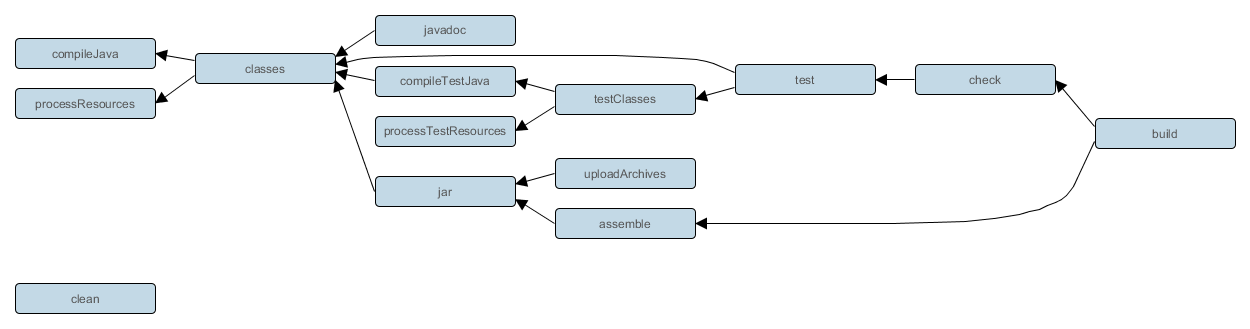
\includegraphics[width=\textwidth]{img/javaPluginTasks}
\end{frame}

\begin{frame}[fragile,allowframebreaks]{Java HelloWorld build}
    \begin{block}{Takeaways}
        \begin{itemize}
            \item Zero configuration required if you follow the convention
        \end{itemize}
    \end{block}
    \terminal{13-Java}{tree before}{\normalsize}
    \groovy{13-Java}{build.gradle}{\normalsize}
    \java{13-Java}{src/main/java/HelloWorld.java}{\normalsize}
    \terminal{13-Java}{gradle clean build}{\scriptsize}
    \terminal{13-Java}{tree after}{\scriptsize}
\end{frame}

\begin{frame}[fragile]{Java libraries as dependencies}
    \begin{itemize}
        \item Java itself has no preferred way for retrieving libraries
        \begin{itemize}
            \item Python got \texttt{pip}
            \item Ruby got \texttt{gem}
            \item Java got nothing
        \end{itemize}
        \item The sole abstraction is classpath
        \begin{itemize}
            \item The list of paths where classes are looked for
            \item Java 9 actually introduces modules, but it doesn't impact the discussion
        \end{itemize}
        \item Apache Ivy first introduced a systematic way of organising java software
        \begin{itemize}
            \item Transitive package manager
            \item Traditionally used along with Ant (imperative build system)
            \item XML-driven declaration of project dependencies and JAR repositories
            \item Quickly got the status of de-facto standard
            \item A library is identified by a triple
            \begin{itemize}
                \item group, artifact, version
            \end{itemize}
        \end{itemize}
        \item The Java Gradle plugin can use repositories in Ivy format
    \end{itemize}
\end{frame}

\begin{frame}[fragile]{OSSRH / The Central Repository}
    \begin{itemize}
        \item The Maven Central Repository\footnote{\url{http://search.maven.org/}} is the most famous repository for open source Java artifacts
        \item Every well known library has artifacts published there
        \item Artifacts are organized in Ivy / Maven format
        \item Safety enforced by a no-retract policy
    \end{itemize}
\end{frame}

\begin{frame}[fragile]{Java dependencies in Gradle}
    \begin{itemize}
        \item Repositories are configured in a \texttt{repositories} block
        \begin{itemize}
            \item Repositories can be specified by URL
            \item Special entries exist for well known repositories
            \begin{itemize}
             \item e.g. \texttt{mavenCentral()}
            \end{itemize}
        \end{itemize}
        \item Dependencies are declared in a \texttt{dependencies} block
        \item Dependencies are identified by an Ivy triple in the format:
        \begin{itemize}
            \item \texttt{\color{blue}group\color{black}:\color{red}artifact\color{black}:\color{olive}version}
            \item e.g. \texttt{\color{blue}it.unibo.alchemist\color{black}:\color{red}alchemist-interfaces\color{black}:\color{olive}7.0.2}
        \end{itemize}
        \item Each \textit{dependency configuration} (build scope) has its own set of dependencies
    \end{itemize}
\end{frame}

\begin{frame}[fragile]{(Some of the) Dependency Configurations}
    \begin{itemize}
        \item \texttt{compileOnly} --- Dependencies required for compiling the project that should not get included at runtime
        \item \texttt{implementation} --- Dependencies required for compiling the project, also required at runtime
        \item \texttt{runtimeOnly} --- Dependencies required for runtime, but not for compiling (e.g. because loaded by reflection)
        \item \texttt{testCompileOnly} --- Dependencies required for compiling tests that should not be included when the tests are executed
        \item \texttt{testImplementation} --- Dependencies required for compiling tests, also required for executing them (e.g. JUnit)
        \item \texttt{testRuntimeOnly} --- Dependencies required at test runtime, but not necessary for compiling the tests
        \item \texttt{annotationProcessor} --- Annotation processors used during compilation. It's an advanced Java feature.
    \end{itemize}
\end{frame}

\begin{frame}[fragile]{Dependency management and source sets}
    For every source set \texttt{\textit{sourceSet}}, the following configurations are automatically generated
    \begin{itemize}
        \item \texttt{\textit{sourceSet}CompileOnly} --- Dependencies required for compiling the source set that should not get included at runtime
        \item \texttt{\textit{sourceSet}Implementation} --- Dependencies required for compiling the source set, also required at runtime
        \item \texttt{\textit{sourceSet}RuntimeOnly} --- Dependencies required for runtime, but not for compiling (e.g. because loaded by reflection)
        \item \texttt{\textit{sourceSet}AnnotationProcessor} --- Annotation processors used during compilation.
    \end{itemize}
\end{frame}

\begin{frame}[fragile]{Dependencies among dependency configurations}
    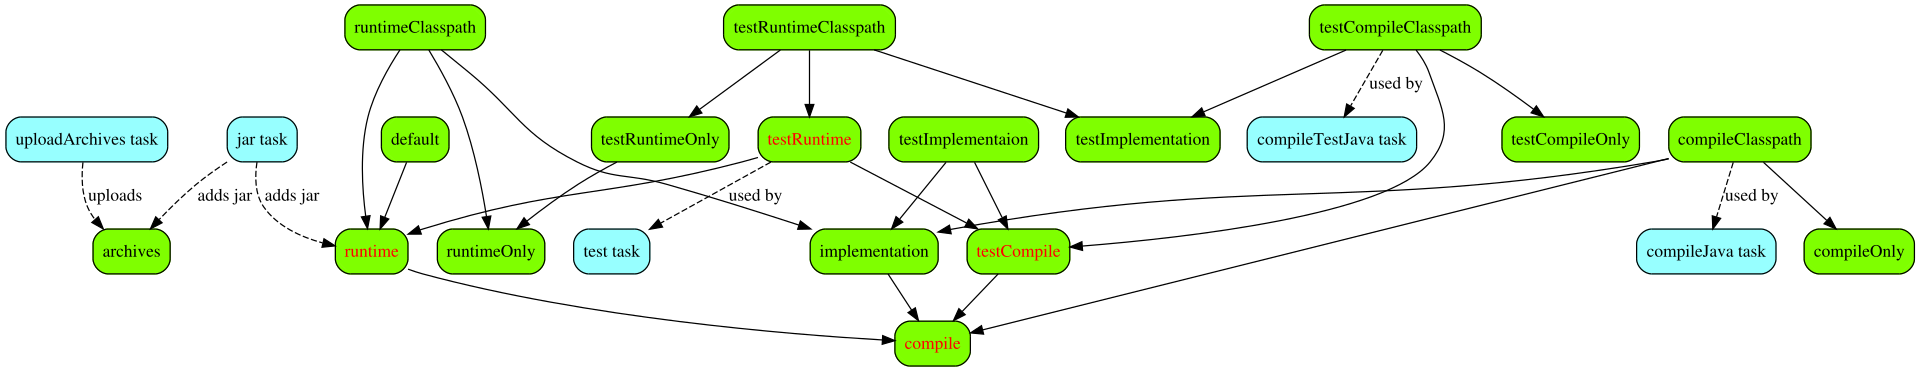
\includegraphics[width=\textwidth]{img/javaPluginConfigurations}
\end{frame}

\begin{frame}[fragile,allowframebreaks]{Java project with dependencies}
    \kotlin{01-dependencies}{src/main/kotlin/it/unibo/ci/PrintSeries.kt}{\tiny}
    \kotlin{01-dependencies}{build.gradle.kts}{\normalsize}
    \kotlin{01-dependencies}{settings.gradle.kts}{\normalsize}
    \begin{block}{Takeaways}
        \begin{itemize}
            \item Using The Central Repository is just matter of a method call
            \item Dependencies are specified per-configuration
            \item \texttt{sourceCompatibility} can be specified to enforce a specific bytecode (and syntax) version
            \item It is a good idea to store properties for the project in the property file
            \item Versions can be specified as exact, ranges, or as latest (risky, don't!)
        \end{itemize}
    \end{block}
\end{frame}

\begin{frame}[fragile,allowframebreaks]{Executing Java programs}
    \java{14-Execution}{src/main/java/it/unibo/ci/PrintBreakingBad.java}{\tiny}
    \groovy{14-Execution}{build.gradle}{\scriptsize}
    \groovy{14-Execution}{gradle.properties}{\scriptsize}
    \groovy{14-Execution}{settings.gradle}{\normalsize}
    \begin{block}{Takeaways}
        \begin{itemize}
            \item It's possible to extend existing task types
            \item An extended task inherits the properties of the parent
        \end{itemize}
    \end{block}
\end{frame}

\subsection{Kotlin, Scala, Groovy, and other JVM languages}

\begin{frame}[fragile]{The JVM ecosystem}
    \begin{block}{The Java Virtual Machine is not for Java}
        \begin{itemize}
            \item The JVM is a \textit{Java bytecode} interpreter
            \item It does not care about which language generated it, as long as it is correct
            \item Java is \textit{one} of the possible languages that compile to Java bytecode
        \end{itemize}
    \end{block}
    \begin{block}{Non-exhaustive list of JVM languages}
        \scriptsize
        \begin{itemize}
            \item \textbf{Ceylon} --- A modernized Java proposed by RedHat
            \item \textbf{Clojure} --- A dialect of LISP
            \item \textbf{Groovy} --- Dynamic programming language
            \item \textbf{JRuby} --- Implementation of Ruby
            \item \textbf{Jython} --- Implementation of Python
            \item \textbf{Kotlin} --- A modernized Java that mixes in some features of functional programming, adopted by Google as official language for Android
            \item \textbf{Scala} --- Advanced, scalable, object-oriented, and functional language
        \end{itemize}
    \end{block}
\end{frame}

\begin{frame}[fragile]{Interoperability among languages}
    \begin{itemize}
        \item Languages that compile on the JVM can usually interoperate
        \begin{itemize}
            \item How well depends on a number of factors
        \end{itemize}
        \item Multiple of them can be used together in a single project
        \item Possibly along other languages, like C/C++ or Javascript
    \end{itemize}
    A well configured build enables using languages as tools, using the right one for the right task
\end{frame}

\begin{frame}[fragile,allowframebreaks]{Example of multilanguage build}
    \java{16-Multilang}{src/main/java/HelloWorld.java}{\normalsize}
    \groovy{16-Multilang}{src/main/groovy/HelloGroovy.groovy}{\normalsize}
    \kotlin{16-Multilang}{src/main/kotlin/HelloKt.kt}{\normalsize}
    \scala{16-Multilang}{src/main/scala/HelloScala.scala}{\normalsize}
    \groovy{16-Multilang}{settings.gradle}{\normalsize}
    \groovy{16-Multilang}{gradle.properties}{\scriptsize}
    \groovy{16-Multilang}{build.gradle}{\tiny}
    \terminal{16-Multilang}{gradle clean build}{\tiny}
    \begin{block}{Takeaways}
        \begin{itemize}
            \item Most of the JVM languages (and all those commonly used) are well supported in Gradle
            \begin{itemize}
                \item Either natively (Scala, Groovy) or via third party plugin (Kotlin)
            \end{itemize}
            \item Multiple languages can coexist in the same project
            \item Your mileage may vary!
            \item It is advisable to divide your project in sub-projects for better interoperability
        \end{itemize}
    \end{block}
\end{frame}

\subsection{C/C++}

\begin{frame}[fragile]{C/C++ and Gradle}
    C and C++ are first class citizens in Gradle
    \begin{block}{Main features}
        \begin{itemize}
            \item No classic dependency management for C could be mimicked
            \begin{itemize}
                \item You are a bit on your own
            \end{itemize}
            \item There is support for several toolchains (in italic the experimental ones)
            \begin{itemize}
                \item GCC and Clang on Linux and \textit{other Unix}
                \item XCode, \textit{GCC (from Macports)}, and \textit{Clang (from Macports)} on MacOS
                \item VisualC++, Cygwin32, \textit{Cygwin64}, and MinGW on Windows
            \end{itemize}
            \item Some care must be provided for cross-compilation
            \item Convention over configuration introduces some unusual ways of organising code
            \begin{itemize}
                \item There are guides for that \footnote{\url{https://bit.ly/2LnKHOz}}
            \end{itemize}
        \end{itemize}
    \end{block}
\end{frame}

\begin{frame}[fragile,allowframebreaks]{Simple C application}
    \ccode{17-C}{src/main/c/greeting.h}{\normalsize}
    \ccode{17-C}{src/main/c/main.c}{\normalsize}
    \groovy{17-C}{settings.gradle}{\normalsize}
    \groovy{17-C}{build.gradle}{\normalsize}
    \begin{block}{Takeaways}
        \begin{itemize}
            \item Native build definitions happen inside a \texttt{model} block
            \item Native executables are defined by a name and a \texttt{NativeExecutableSpec}
        \end{itemize}
    \end{block}
\end{frame}

\begin{frame}[fragile,allowframebreaks]{Simple C++ application}
    \ccode{18-CPP}{src/main/cpp/greeting.hpp}{\normalsize}
    \ccode{18-CPP}{src/main/cpp/main.cpp}{\normalsize}
    \groovy{18-CPP}{settings.gradle}{\normalsize}
    \groovy{18-CPP}{build.gradle}{\normalsize}
    \begin{block}{Takeaways}
        \begin{itemize}
            \item Basically the same thing as building plain C
            \item In fact the toolchain is basically unified
        \end{itemize}
    \end{block}
\end{frame}

\begin{frame}[fragile]{Advanced examples}
    Gradle has rich documentation on building native software:
    \begin{itemize}
        \item Documentation on building native software \footnote{\url{https://docs.gradle.org/4.7/userguide/native_software.html}}
        \item Building C/C++ libraries \footnote{\url{https://guides.gradle.org/building-cpp-libraries/}}
        \item A repository of examples in C, C++, and Swift \footnote{\url{https://github.com/gradle/native-samples}}
    \end{itemize}
\end{frame}

\subsection{Other languages}

\begin{frame}[fragile]{Python}
    Python provides native tools for environment configuration, dependency management, and packaging, making Gradle largely unnecessary
    \begin{itemize}
        \item Still, a third party plugin is provided by LinkedIn\fnurl{https://github.com/linkedin/pygradle}
        \item Converts PyPI data in Ivy format
        \item LinkedIn published an Ivy-compatible repository of all the code on PyPI
    \end{itemize}
    \begin{block}{Recommended tools}
        \begin{itemize}
            \item Python natively promotes working in virtual environments
            \item PyPI is a Python software repository (the Python equivalent of Maven Central)
            \item \texttt{pip} is a command line tool for pulling packaging from PyPI
            \item \texttt{setuptools} provides building and packaging capabilities
        \end{itemize}
    \end{block}
\end{frame}    
\begin{frame}[fragile]{Working with Python virtual environments}
    A virtual environment for Python isolates application-specific dependencies from a shared (system-wide) python installation
    \begin{itemize}
        \item Python 3.4+ is shipped with the capability of creating a virtual environment with the \texttt{pip} package manager pre-installed
        \item A new virtual environment can be created by issuing:
        \begin{itemize}
            \item \texttt{python -m venv \textit{foldername}}
        \end{itemize}
        \item Once created, a virtual environment can be entered in using:
        \begin{itemize}
            \item \texttt{source \textit{foldername}/bin/activate}
        \end{itemize}
        \item Commands issued within an activate shell will be executed in the virtual environment
        \begin{itemize}
            \item e.g. \texttt{pip install xarray} would install xarray in the virtual environment, not system wide.
        \end{itemize}
        \item This enables controlling dependencies' versions
        \item To get back to a normal shell, issue the command \texttt{deactivate}
    \end{itemize}
\end{frame}

\begin{frame}[fragile]{C\# and .NET}
    Support or C\# and other .NET languages is rather faltering
    \begin{itemize}
        \item There is an open discussion \fnurl{https://github.com/gradle/gradle/issues/1428} about supporting .NET in a more official way
        \item Currently, the best solution is using a third party plugin: \fnurl{https://github.com/Ullink/gradle-msbuild-plugin}
        \begin{itemize}
            \item Controls \texttt{msbuild} through Gradle
        \end{itemize}
    \end{itemize}
\end{frame}

\subsection{Automated QA}

\begin{frame}[fragile]{QA and research}
    Research projects must not be considered ``immune'' to QA problems
    \begin{block}{Common issues}
    \footnotesize
        \begin{itemize}
            \item \textit{Reproducibility} --- Software/experiment results are inconsistent or non-reproducible
            \item \textit{Communicability} --- The software quality makes it hard to to understand and contribute, even within the development team
            \item \textit{Availability} --- Research tools are not properly packed and shared, and as such the rest of the community can not exploit them appropriately
            \item \textit{Scaling} --- Many research projects that may aim to industrial applications won't be able to without proper QA
            \item \textit{Consistency} --- The project is written using an inconsistent style, that poses a barrier to understanding and contribution. This is especially true for teams
        \end{itemize}
    \end{block}
    \begin{itemize}
        \item Software QA is very time-consuming, performing it manually may jeopardize the short term success of a research project
        \begin{itemize}
            \item Possibly impacting publications negatively
        \end{itemize}
        \item Automatization trades an upfront cost for a long term benefit
    \end{itemize}
\end{frame}

\begin{frame}[fragile]{The importance of testing}
    Your project should \textbf{always} have some tests
    \begin{block}{Why is testing software necessary}
        \begin{itemize}
            \item \textit{Quality assurance} --- Critical parts of the system can be stressed to verify their conformance
            \item \textit{Bug hunting} --- Reproducing bug in a controlled setup helps with quick resolution
            \item \textit{Error tracking} --- If a test is introduced for every defect discovered during development, a clear trace of errors is maintained
            \item \textit{Regression prevention} --- A good test suite prevents working features to be compromised by further development
        \end{itemize}
    \end{block}
    \begin{block}{Why testing must be automated}
        \begin{itemize}
            \item \textit{Saves time} --- manual execution is time expensive
            \item \textit{Consistency} --- manual execution could be not always performed
        \end{itemize}
    \end{block}
\end{frame}

\begin{frame}[fragile]{JUnit}
    JUnit is one of the most famous frameworks for testing Java software
    \begin{itemize}
        \item Unit testing is a in-the-small testing
        \begin{itemize}
            \item Though the library is often abused to go well past units
        \end{itemize}
        \item Details are not part of the course
        \item If you are a java developer and are not using Junit, \textbf{learn it!}
        \item The Java Plugin for Gradle includes a nice support for Junit testing
        \item Ancillary frameworks can be used in conjunction JUnit to implement advanced features
        \begin{itemize}
            \item Test Doubles (dummies, stubs, fakes, spies, mocks)
            \item Performance / scalability test
            \item Microbenchmarking
            \item Browser based testing
            \item ...
        \end{itemize}
    \end{itemize}
\end{frame}

\begin{frame}[fragile,allowframebreaks]{Test automation with Gradle and JUnit}
    \java{15-Test}{src/main/java/POJO.java}{\tinier}
    \java{15-Test}{src/test/java/TestPOJO.java}{\tinier}
    \groovy{15-Test}{gradle.properties}{\scriptsize}
    \groovy{15-Test}{build.gradle}{\scriptsize}
    \groovy{15-Test}{settings.gradle}{\normalsize}
    \terminal{15-Test}{gradle clean build}{\tiny}
    \centering
    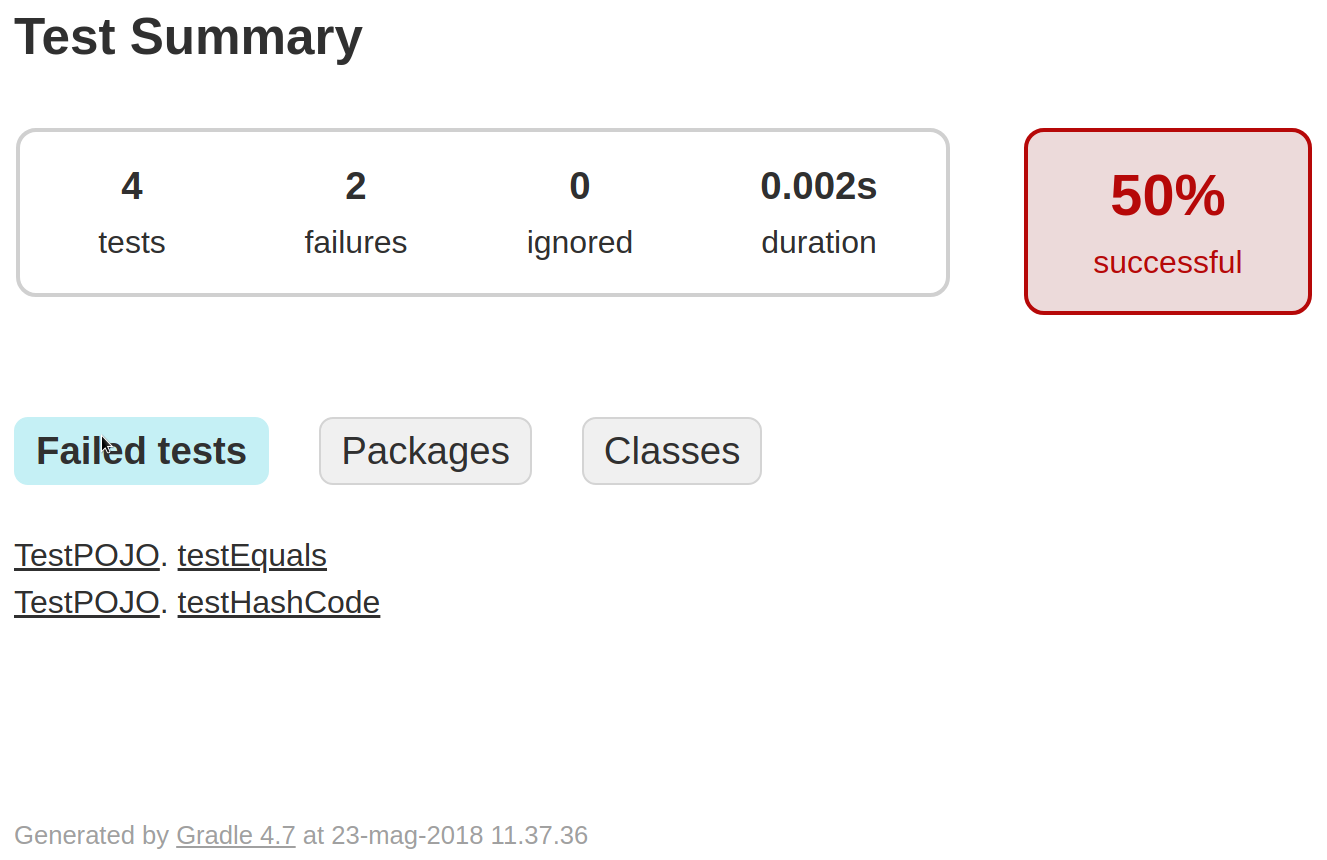
\includegraphics[width=.9\textwidth,height=.8\textheight,keepaspectratio]{img/gradleTestReport0}
    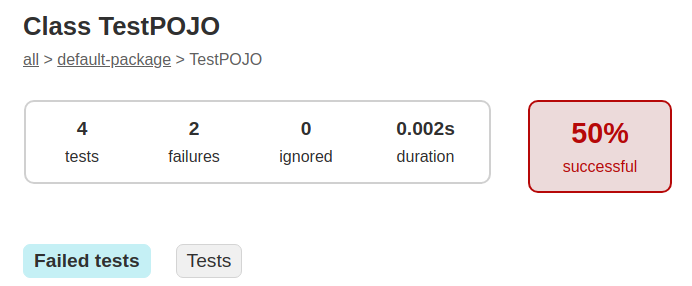
\includegraphics[width=.9\textwidth,height=.8\textheight,keepaspectratio]{img/gradleTestReport1}
    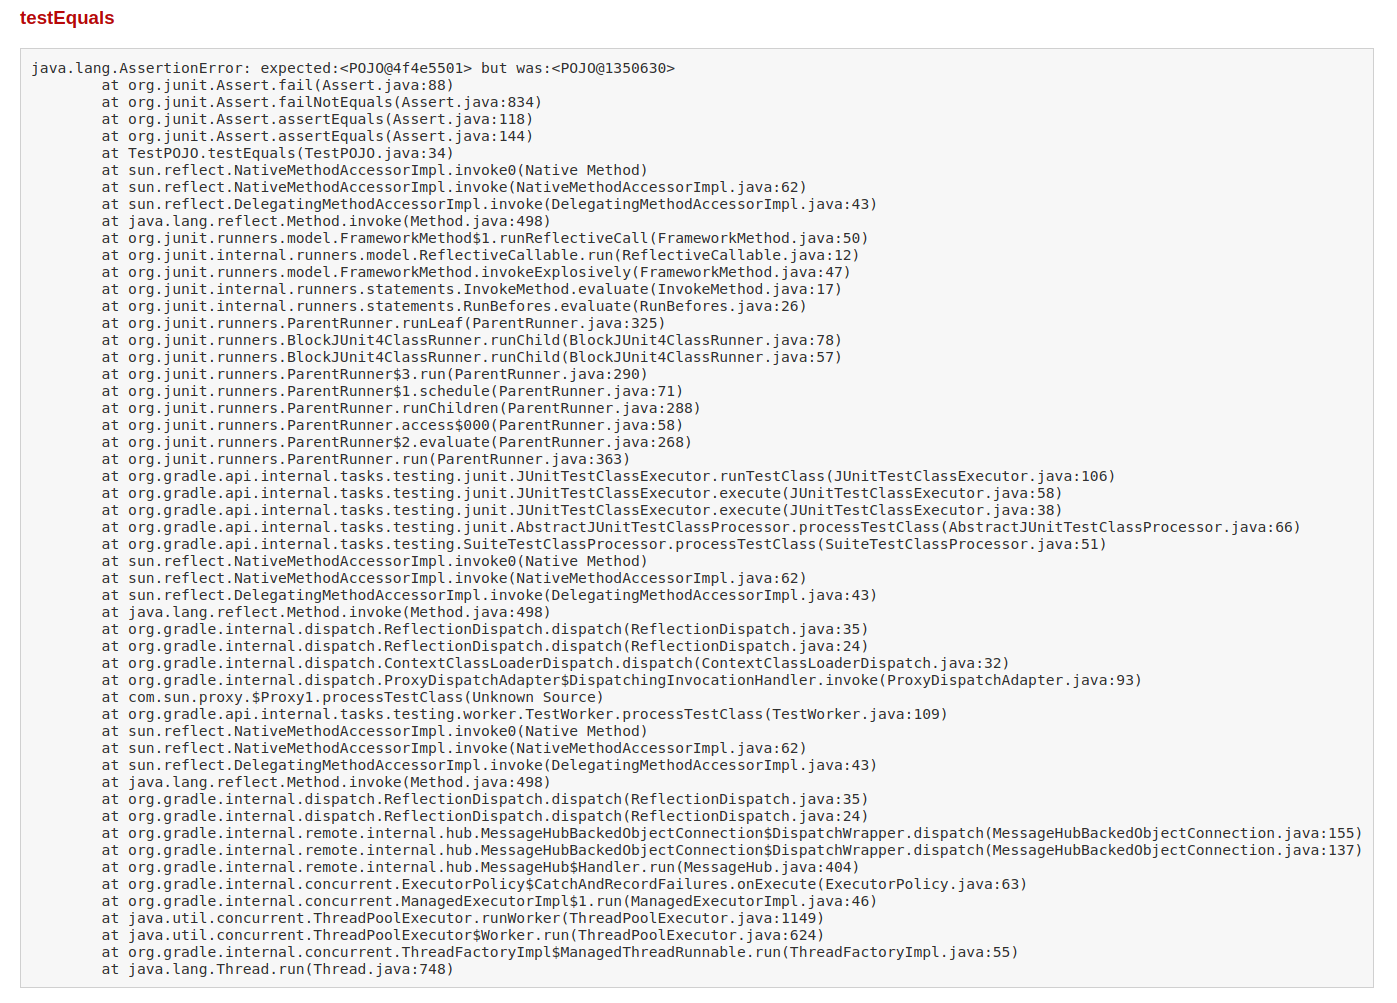
\includegraphics[width=.9\textwidth,height=.8\textheight,keepaspectratio]{img/gradleTestReport2}
    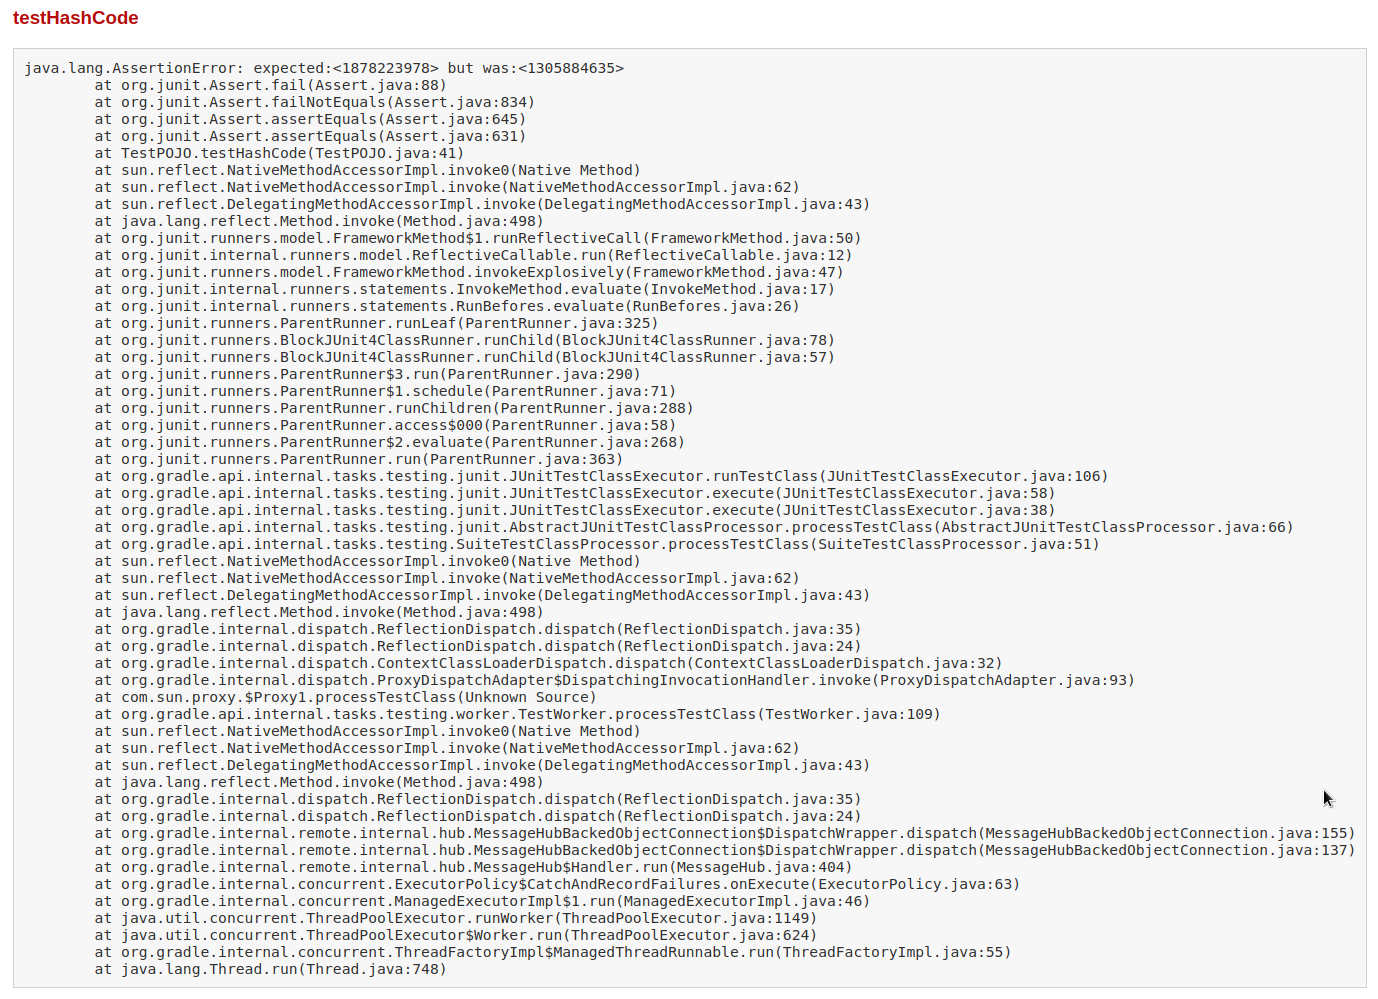
\includegraphics[width=.9\textwidth,height=.8\textheight,keepaspectratio]{img/gradleTestReport3}
    \begin{block}{Takeaways}
        \begin{itemize}
            \item If JUnit is included in the test classpath, the execution of tests is automatic
            \item Tests are performed at every build
            \item A report is automatically produced
            \item A description of the failures is included in the report
        \end{itemize}
    \end{block}
\end{frame}

\begin{frame}[fragile, allowframebreaks]{Other frameworks}
    \begin{block}{C}
        CUnit\footnote{\url{http://cunit.sourceforge.net/}} is natively supported:
        \begin{minted}{groovy}
apply plugin: 'cunit-test-suite'
        \end{minted}
    \end{block}
    \begin{block}{C++}
        Google Test\footnote{\url{https://github.com/google/googletest}} is natively supported:
        \begin{minted}{groovy}
apply plugin: 'google-test'
        \end{minted}
    \end{block}
    \begin{block}{Javascript}
        Third party plugin\fnurl{https://github.com/dzhaughnroth/jasmine-gradle-plugin} available for Jasmine\footnote{\url{https://jasmine.github.io/}}.
    \end{block}
\end{frame}

\begin{frame}[fragile]{Test coverage}
    Test coverage detects:
    \begin{itemize}
        \item The amount of lines of codes actually tested
        \item The number of branches explored when executing tests
        \item \textit{Which} lines of code have been tested
        \item \textit{Which} branches of code have been tested
    \end{itemize}
    It can be used as a measure of test quality, and in turn as a measure of software quality \cite{Horgan1994}, but be aware that high coverage does not automatically mean high quality software \cite{Inozemtseva2014}. 
\end{frame}

\begin{frame}[fragile]{Test when needed, use coverage critically}
    \begin{block}{What coverage actually tells you}
        If you have X\% coverage, you have \textit{at least} 100-X\% uncovered statements
    \end{block}
    Good practices
    \begin{itemize}
        \item When you are working on a new feature, write an automatic test in place of testing it manually
        \begin{itemize}
            \item If you don't get it right at the first attempt, you will save development time
            \item You get a free regression test for the future
        \end{itemize}
        \item Every time you walk into a bug, before fixing it write a test that
        \begin{itemize}
            \item Systematically fails if the bug is still there
            \item Systematically passes if the bug is not there
        \end{itemize}
        \item Use coverage to spot parts of your software that are untested
        \item Enforcing a coverage level may help with lazy collaborators, but won't automatically raise your software quality
        \item Do not bask in the glory of a high coverage
    \end{itemize}
\end{frame}

\begin{frame}[fragile]{Coverage in Gradle}
    \begin{itemize}
        \item Coverage tools must understand the language code and tests are written in
        \begin{itemize}
            \item You must pick the right tool for the code you are writing
        \end{itemize}
        \item Gradle integrates the JaCoCo plugin for Java (also covers Scala and Kotlin, but may be less precise)
        \item Third-party plugins are available for the same and other languages:
        \begin{itemize}
            \item Cobertura for Java \fnurl{https://github.com/stevesaliman/gradle-cobertura-plugin}
            \item Scoverage for Scala \fnurl{https://github.com/scoverage/gradle-scoverage}
        \end{itemize}
    \end{itemize}
\end{frame}

\begin{frame}[fragile,allowframebreaks]{Coverage with Gradle and JaCoCo}
    \java{19-Coverage}{src/main/java/POJO.java}{\tinier}
    \java{19-Coverage}{src/test/java/TestPOJO.java}{\tinier}
    \groovy{19-Coverage}{gradle.properties}{\scriptsize}
    \groovy{19-Coverage}{build.gradle}{\scriptsize}
    \groovy{19-Coverage}{settings.gradle}{\normalsize}
    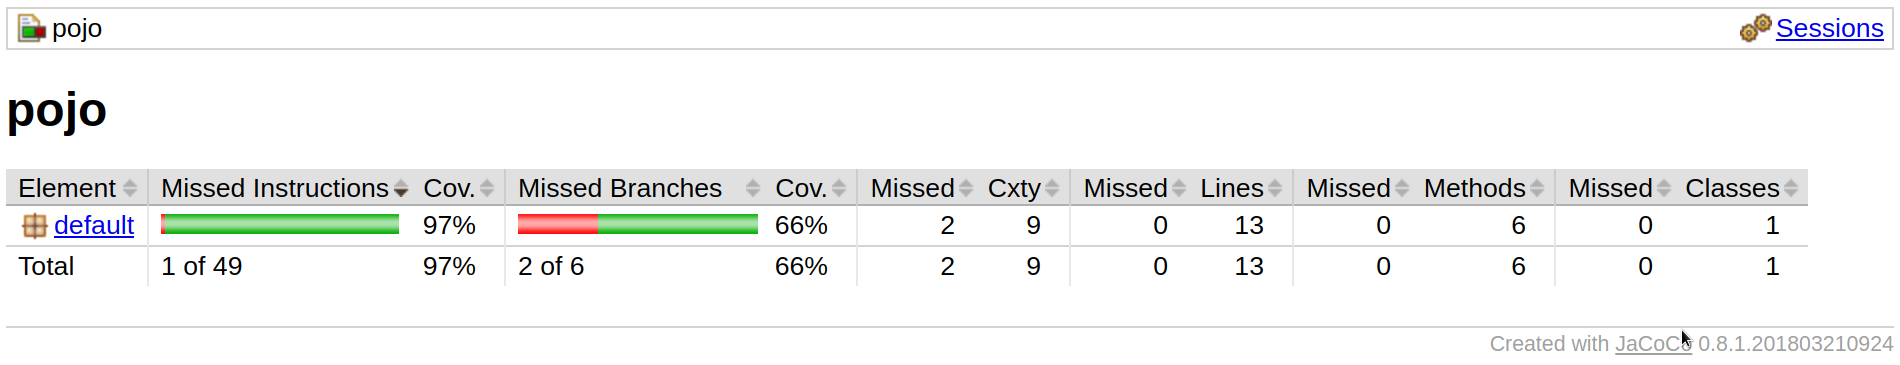
\includegraphics[width=.9\textwidth,height=.8\textheight,keepaspectratio]{img/jacocoTestReport0}
    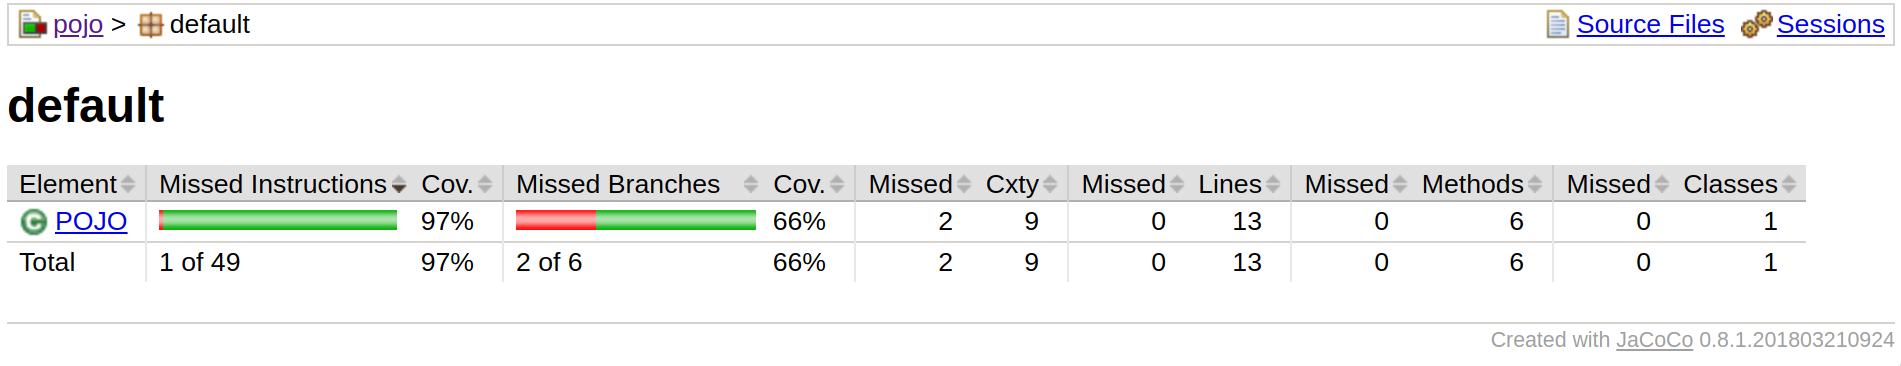
\includegraphics[width=.9\textwidth,height=.8\textheight,keepaspectratio]{img/jacocoTestReport1}
    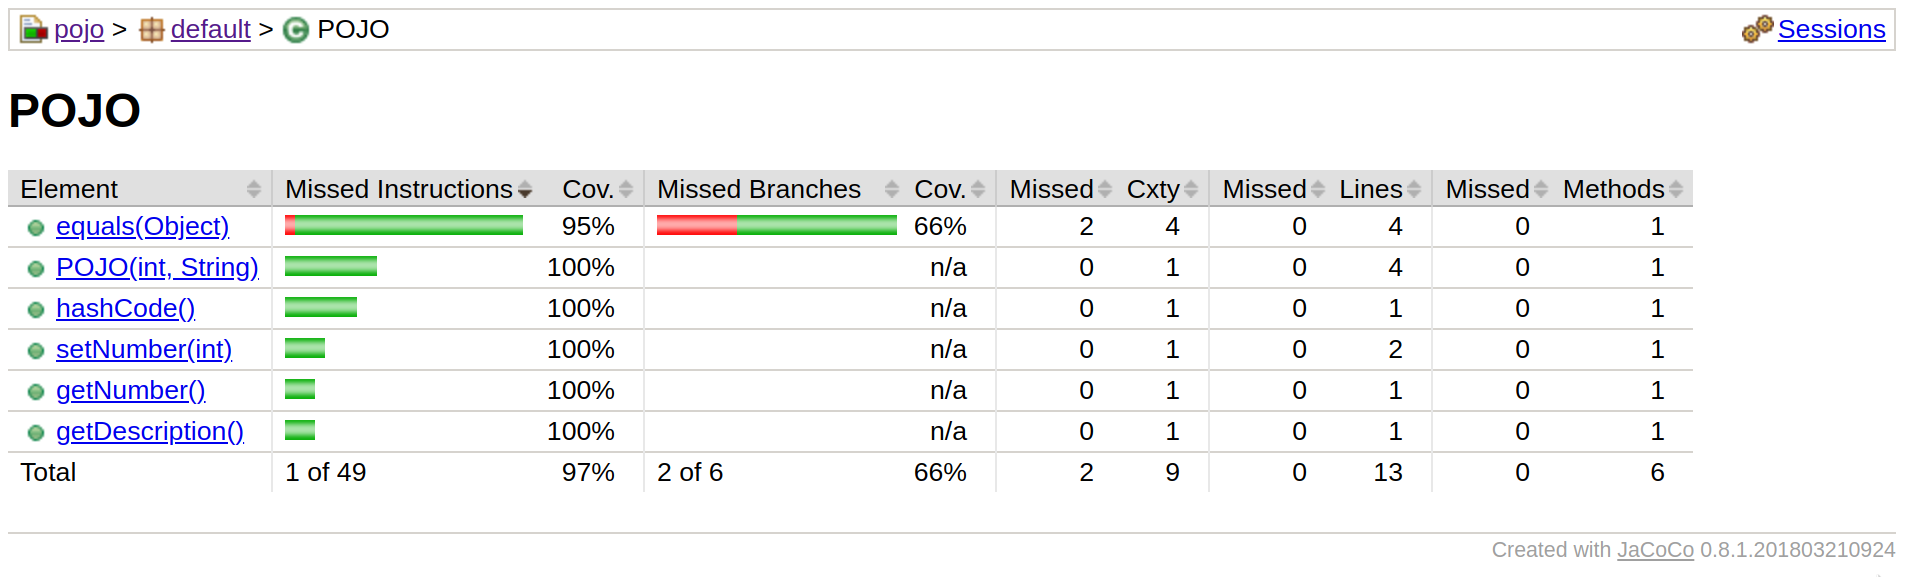
\includegraphics[width=.9\textwidth,height=.8\textheight,keepaspectratio]{img/jacocoTestReport3}
    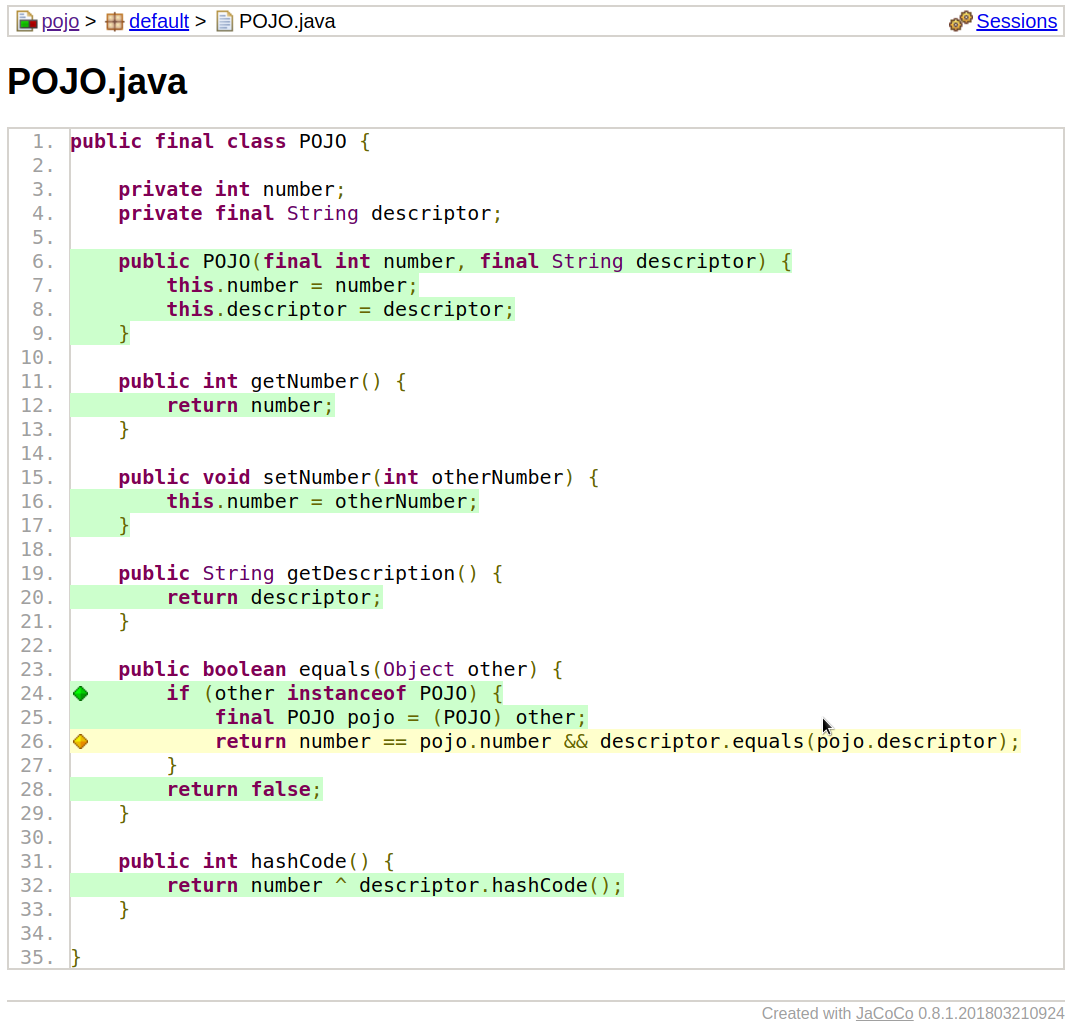
\includegraphics[width=.9\textwidth,height=.8\textheight,keepaspectratio]{img/jacocoTestReport4}
\end{frame}

\begin{frame}[fragile]{Enforcing code conventions}
    Tools that enforce code conventions help in:
    \begin{itemize}
        \item Spot bugs early by scanning the code for common mistakes
        \item Spot performance pitfalls early by scanning the code for common mistakes
        \item Intercept practices correct in general but wrong for the specific project
        \begin{itemize}
            \item e.g. calling an external random in a simulator (breaks reproducibility)
        \end{itemize}
        \item Raise the understandability of the code by making it looking homogeneous
        \item Nullify the possibility of having big changesets for minimal actual changes
        \begin{itemize}
            \item e.g. because different developers use systems with different newlines
        \end{itemize}
        \item Raise the communicability of the code by following a set of rules shared by the community
        \item Produce a report with an indication of the points where code has the lowest quality
    \end{itemize}
\end{frame}

\begin{frame}[fragile, allowframebreaks]{Code checking tools by language}
    \begin{block}{C}
        \begin{itemize}
            \item Artistic Style\fnurl{http://astyle.sourceforge.net/}
            \item GNU Indent\fnurl{http://www.gnu.org/software/indent/}
            \item Infer\fnurl{http://fbinfer.com/}
            \item nsiqcppstyle\fnurl{https://code.google.com/archive/p/nsiqcppstyle/}
            \item Uncrustify\fnurl{http://uncrustify.sourceforge.net/}
        \end{itemize}
    \end{block}
    \begin{block}{C++}
        \begin{itemize}
            \item Artistic Style\fnurl{http://astyle.sourceforge.net/}
            \item cpplint\fnurl{https://github.com/google/styleguide/tree/gh-pages/cpplint}
            \item KWStyle\fnurl{http://kitware.github.io/KWStyle/}
            \item Infer\fnurl{http://fbinfer.com/}
            \item Uncrustify\fnurl{http://uncrustify.sourceforge.net/}
            \item Vera++\fnurl{https://bitbucket.org/verateam/vera/wiki/Home}
        \end{itemize}
    \end{block}
    \begin{block}{C\#}
        \begin{itemize}
            \item Artistic Style\fnurl{http://astyle.sourceforge.net/}
            \item StyleCop\fnurl{https://github.com/StyleCop}
            \item Uncrustify\fnurl{http://uncrustify.sourceforge.net/}
        \end{itemize}
    \end{block}
    \begin{block}{Go}
        \begin{itemize}
            \item CPD\fnurl{https://pmd.github.io/}
            \item (Go)Checkstyle\fnurl{https://github.com/qiniu/checkstyle}
        \end{itemize}
    \end{block}
    \begin{block}{Java}
        \begin{itemize}
            \item Artistic Style\fnurl{http://astyle.sourceforge.net/}
            \item Checkstyle\fnurl{http://checkstyle.sourceforge.net/}
            \item Infer\fnurl{http://fbinfer.com/}
            \item PMD/CPD\fnurl{https://pmd.github.io/}
            \item SpotBugs\fnurl{https://spotbugs.github.io/}
            \item Uncrustify\fnurl{http://uncrustify.sourceforge.net/}
        \end{itemize}
    \end{block}
    \begin{block}{Javascript}
        \begin{itemize}
            \item CPD\fnurl{https://pmd.github.io/}
            \item ESLint\fnurl{https://eslint.org/}
            \item StandardJS\fnurl{https://standardjs.com/}
        \end{itemize}
    \end{block}
    \begin{block}{Kotlin}
        \begin{itemize}
            \item Klint\fnurl{https://github.com/shyiko/ktlint}
            \item Detekt\fnurl{https://github.com/arturbosch/detekt}
        \end{itemize}
    \end{block}
    \begin{block}{Matlab}
        \begin{itemize}
            \item CPD\fnurl{https://pmd.github.io/}
            \item Matlab Code Analyzer\fnurl{https://github.com/bastibe/MatlabCodeAnalyzer}
            \item MStyle\fnurl{https://github.com/KEClaytor/MStyle}
        \end{itemize}
    \end{block}
    \begin{block}{PHP}
        \begin{itemize}
            \item CPD\fnurl{https://pmd.github.io/}
            \item phlint\fnurl{https://gitlab.com/phlint/phlint}
            \item PHP Mess Detector\fnurl{https://phpmd.org/}
            \item progpilot\fnurl{https://github.com/designsecurity/progpilot}
        \end{itemize}
    \end{block}
    \begin{block}{Objective-C}
        \begin{itemize}
            \item Artistic Style\fnurl{http://astyle.sourceforge.net/}
            \item CPD\fnurl{https://pmd.github.io/}
            \item Infer\fnurl{http://fbinfer.com/}
            \item Uncrustify\fnurl{http://uncrustify.sourceforge.net/}
        \end{itemize}
    \end{block}
    \begin{block}{Python}
        \begin{itemize}
            \item CPD\fnurl{https://pmd.github.io/}
            \item pycodestyle (formerly pep8)\fnurl{https://github.com/PyCQA/pycodestyle}
            \item Pyflakes\fnurl{https://github.com/PyCQA/pyflakes}
            \item Pylint\fnurl{https://www.pylint.org/}
            \item Vera++\fnurl{https://bitbucket.org/verateam/vera/wiki/Home}
        \end{itemize}
    \end{block}
    \begin{block}{Ruby}
        \begin{itemize}
            \item CPD\fnurl{https://pmd.github.io/}
            \item RuboCop\fnurl{https://github.com/bbatsov/rubocop}
        \end{itemize}
    \end{block}
    \begin{block}{Scala}
        \begin{itemize}
            \item Scalastyle\fnurl{http://www.scalastyle.org/}
            \item CPD\fnurl{https://pmd.github.io/}
        \end{itemize}
    \end{block}
    \begin{block}{Swift}
        \begin{itemize}
            \item CPD\fnurl{https://pmd.github.io/}
            \item SwiftLint\fnurl{https://github.com/realm/SwiftLint}
        \end{itemize}
    \end{block}
\end{frame}

\begin{frame}[fragile,allowframebreaks]{Checking code quality with Checkstyle and Gradle}
    \java{20-Checkstyle}{src/main/java/POJO.java}{\tinier}
    \java{20-Checkstyle}{src/test/java/TestPOJO.java}{\tinier}
    \groovy{20-Checkstyle}{gradle.properties}{\scriptsize}
    \groovy{20-Checkstyle}{build.gradle}{\scriptsize}
    \groovy{20-Checkstyle}{settings.gradle}{\normalsize}
    \begin{block}{\texttt{config/checkstyle/checkstyle.xml}}
        \inputminted[fontsize=\tiny,linenos=true,breaklines=true,firstline=1,lastline=25]{xml}{workspace/20-Checkstyle/config/checkstyle/checkstyle.xml}
    \end{block}
\end{frame}

\begin{frame}[fragile]{Generating dashboards}
    \begin{itemize}
        \item A well organized project has a number of reports
        \begin{itemize}
            \item Test results
            \item Test coverage
            \item Several code quality reports (different tools inspect different aspects)
        \end{itemize}
        \item Each report stands alone by default
        \item A dashboard provides an entry point for all the reports produced by QA tools
        \item Gradle includes a default Build Dashboard plugin
        \begin{itemize}
            \item The plugin is currently \textit{incubating}
        \end{itemize}
    \end{itemize}
\end{frame}

\begin{frame}[fragile,allowframebreaks]{Generating a dashboard with all project reports}
    \java{21-Dashboard}{src/main/java/POJO.java}{\tinier}
    \java{21-Dashboard}{src/test/java/TestPOJO.java}{\tinier}
    \begin{block}{\texttt{config/checkstyle/checkstyle.xml}}
        \inputminted[fontsize=\tiny,linenos=true,breaklines=true,firstline=1,lastline=25]{xml}{workspace/21-Dashboard/config/checkstyle/checkstyle.xml}
    \end{block}
    \groovy{21-Dashboard}{gradle.properties}{\scriptsize}
    \groovy{21-Dashboard}{settings.gradle}{\normalsize}
    \groovy{21-Dashboard}{build.gradle}{\scriptsize}
\end{frame}

\begin{frame}[fragile]{Gradle build scans}
    \begin{itemize}
        \item A rich build quickly escalates in complexity
        \item As we want reports to inspect the quality and issues of the project, we'd like a tool to provide better presentation of the build process itself
        \item e.g. for improving performance
        \item gradle provides ``Build Scans'' to tackle this issue
        \item Produces a build report and publishes it online
        \item The \texttt{--scan} option enables the features
        \item A plugin exists to prevent the shell to interactively ask to accept the license agreement
    \end{itemize}
    \begin{block}{Build scans}
        A build scan is a shareable and centralized record of a build that provides insights into what happened and why.
    \end{block}
\end{frame}

\begin{frame}[fragile,allowframebreaks]{Generating and publishing a build scan}
    \groovy{22-Scans}{gradle.properties}{\scriptsize}
    \groovy{22-Scans}{settings.gradle}{\normalsize}
    \groovy{22-Scans}{build.gradle}{\tiny}
    \begin{block}{}
        The result is available at\\ \url{https://scans.gradle.com/s/qd2mieqffudwk}
    \end{block}
\end{frame}

\subsection{Automated documentation and packaging}

\begin{frame}[fragile]{Documenting code and generating API documentation}
    A project should always be shipped with proper documentation
    \begin{itemize}
        \item Most documentation must be prepared manually
        \begin{itemize}
            \item Readmes
            \item Tutorials
            \item Quickstarts
            \item Guides
        \end{itemize}
        \item The API documentation can often be deduced by proper code comments
        \item Tools exist that parse code and produce human-accessible API documentation
        \begin{itemize}
            \item Java's javadoc
            \item Scala's Scaladoc
            \item Kotlin's Dokka
            \item Python's docstrings
            \item ...
        \end{itemize}
    \end{itemize}
\end{frame}

\begin{frame}[fragile]{Generating API documentation with Gradle}
    \begin{itemize}
        \item The methodology varies with languages
        \begin{itemize}
            \item The Java plugin has a built in \texttt{javadoc} task
            \item The \texttt{build} task can be declared dependent from javadoc to automate the generation
            \item Other languages may require a different configuration
            \item e.g. Dokka has a third party plugin, not included in the Kotlin plugin
        \end{itemize}
    \end{itemize}
\end{frame}

\begin{frame}[fragile]{Packaging software}
    \begin{itemize}
        \item A bunch of scripts or binaries is usually not a good way to distribute software
        \item Practices differ by languages and project types:
        \begin{itemize}
            \item In the JVM ecosystem, usually libraries get published along with Ivy-style metadata
            \item JVM-based stand-alone programs are shipped as ``fat jar''
            \begin{itemize}
                \item A jar file containing not just the software itself, but all its dependencies, in such a way that it can get executed on any standard JVM installation
            \end{itemize}
            \item In Python, setuptools is used to package software
        \end{itemize}
    \end{itemize}
\end{frame}

\begin{frame}[fragile, allowframebreaks]{Generating Ivy and Maven compatible metadata in Gradle}
    While a library jar is automatically produced by the \texttt{jar} task of the Java plugin, the companion Ivy metadata is not by default
    \begin{itemize}
        \item A maven plugin is distributed with the tool
        \item It provides a factory for pom files
        \item It provides an \texttt{uploadArchives} task for preparing a Maven-compatible distribution
        \begin{itemize}
            \item Including a valid POM descriptor
        \end{itemize}
    \end{itemize}
    \groovy{23-POM}{gradle.properties}{\scriptsize}
    \groovy{23-POM}{build.gradle}{\tinier}
\end{frame}

\begin{frame}[fragile, allowframebreaks]{Generating a ``fat jar'' in Gradle}
    A fat jar:
    \begin{itemize}
        \item Includes all the libraries required \textit{at runtime}
        \item Is executable
        \begin{itemize}
            \item i.e. has a MANIFEST.MF file indicating the class to execute
        \end{itemize}
    \end{itemize}
    No default task is provided, we need to write one manually extending the existing \texttt{jar}
    \groovy{24-Fatjar}{gradle.properties}{\scriptsize}
    \groovy{24-Fatjar}{build.gradle}{\tinier}
\end{frame}

\begin{frame}[fragile, allowframebreaks]{DVCS-Sensible build}
    You may want the build system to automatically detect the project version from the DVCS and act accordingly
    \begin{itemize}
        \item e.g. if it is tagged and sits on main, it is a release
        \item Otherwise, it is a beta, and we may want to identify it
        \item No direct support in Gradle 
        \begin{itemize}
            \item But you can use a full fledged programming language as Groovy...
            \item And there exist a GrGit library for interacting with git!
        \end{itemize}
    \end{itemize}
    \groovy{26-Git}{settings.gradle}{\scriptsize}
    \groovy{26-Git}{gradle.properties}{\scriptsize}
    \groovy{26-Git}{build.gradle}{\tiny}
\end{frame}

\begin{frame}[fragile,allowframebreaks]{Packaging with Python setuptools}
    Python provides setuptools for easily packaging your software
    \begin{enumerate}
        \item Create your project. In this case, We create just an empty package:
        \python{25-setuptools}{my\string_pkg/\string_\string_init\string_\string_.py}{\normalsize}
        \item Create a valid \texttt{README.md} (GitHub flavored Markdown syntax is supported!)
        \terminal{25-setuptools}{README.md}{\scriptsize}
        \item Create a \texttt{LICENSE} file
        \terminal{25-setuptools}{LICENSE}{\scriptsize}
        \item Create a \texttt{setup.py} file, along the line of:
        \python{25-setuptools}{setup.py}{\tiny}
        \item Create a virtual environment, by issuing: \\
        \texttt{python -m venv venv}
        \item Activate the virtual environment: \\
        \texttt{source venv/bin/activate}
        \item Upgrade pip: \\
        \texttt{pip install pip --upgrade}
        \item Install setuptools and wheel: \\
        \texttt{pip install --upgrade setuptools wheel}
        \item Generate the package! \\
        \texttt{python setup.py sdist bdist\string_wheel}
        \item Deactivate the virtual environment! \\
        \texttt{deactivate}
        \item Packages will be available in the \texttt{dist} folder
    \end{enumerate}
\end{frame}

\section*{\refname}
%===============================================================================
\begin{frame}[allowframebreaks]
  \frametitle{\refname}
  \scriptsize 
  \bibliographystyle{alpha}
  \bibliography{../bibliography}
\end{frame}
\section*{\refname}


\end{document}
